\subsection{MEX 3-1: CNL direct shear test data (TUBAF)}\label{DataManMex3-1CNL}\index{Constant Normal Load (CNL) experiment}

Data management for MEX 3-1 (see \ref{sec:mex07}).

Link to the data set at UFZ data investigation portal: \url{https://www.ufz.de/record/dmp/archive/7925/}

The CNL data set contains four text files. One text file with the rock properties of the used granite (see Tab. \ref{table:MEX7_rockParam}). Two files with the scan data of the two surfaces. One point cloud can be seen in Fig. \ref{fig:DataCNLGranitePointCloud}. The last file contains the laboratory data. In Fig. \ref{fig:DataCNLGraniteLab} the results for the four shear stress levels can be seen.

\begin{figure}[!ht]
\begin{center}
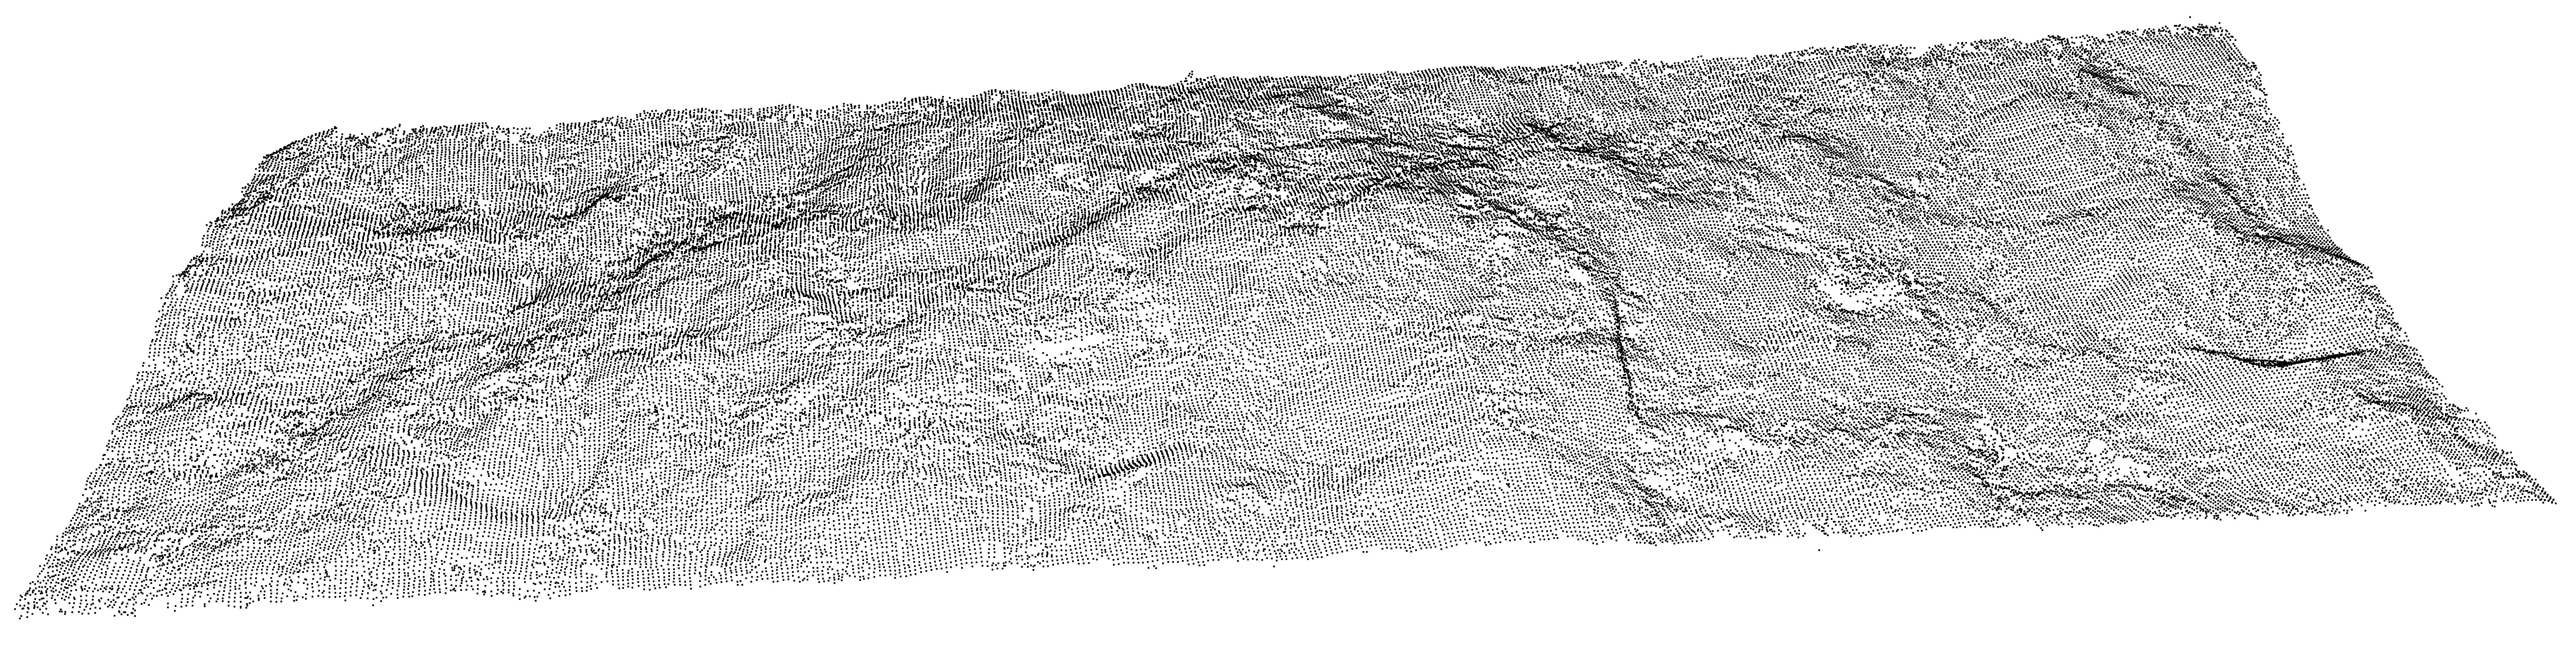
\includegraphics[width=0.75\textwidth]{./figures/MEX7_Point_cloud.png}
\end{center}
\caption{Point cloud representing the surface of a granite sample from Saxony. The size is 65 mm by 170 mm and the cloud contains approx. 98000 points.}
\label{fig:DataCNLGranitePointCloud}
\end{figure}

\begin{figure}[!ht]
\begin{tabular}{cc}
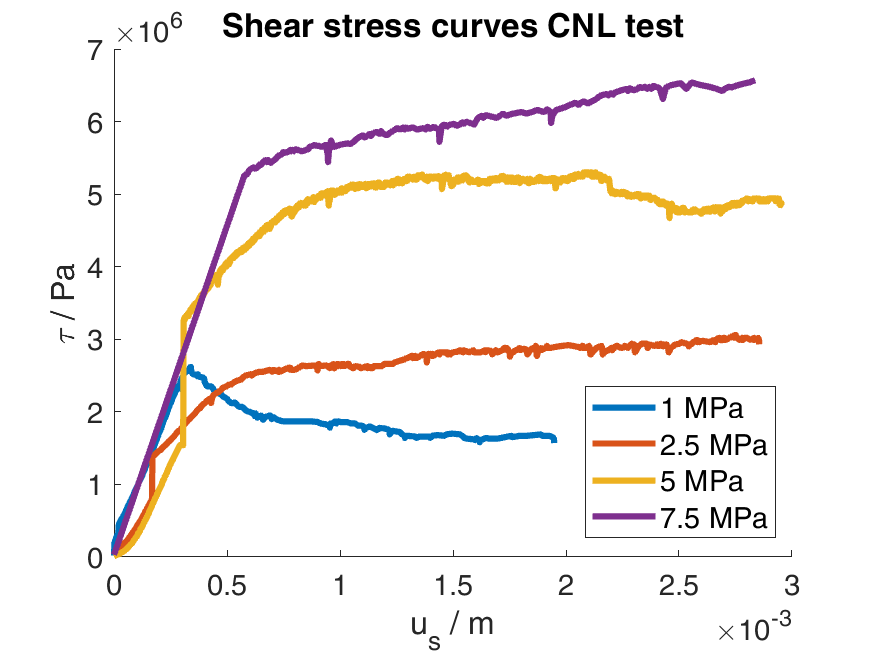
\includegraphics[width=0.45\textwidth]{./figures/CNLShearCurvesAll.png}     
& 
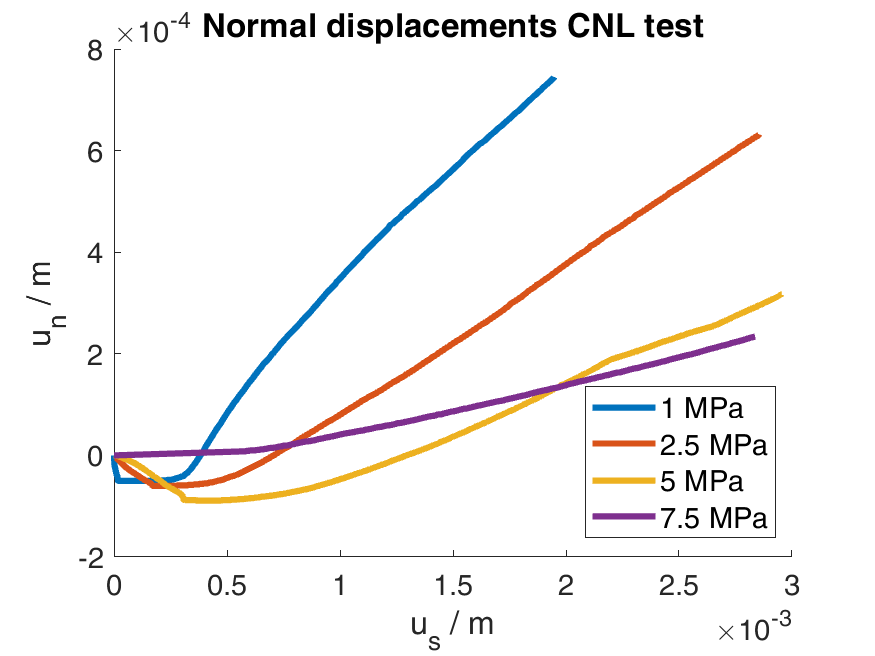
\includegraphics[width=0.45\textwidth]{./figures/CNLDilatationAll.png} 
\end{tabular}
\caption{CNL test results}
\label{fig:DataCNLGraniteLab}
\end{figure}

\begin{table}[!ht]
\caption{MEX 3-1: Meta Data according to Dublin Core}
\label{tab:dms-mex3-1}
\small
\begin{tabular}{R{3cm}|L{7cm}}
\hline
%\rowcolor{Cyan}
%
Data label & GeomInt | TUBAF | Data Set CNL \\
URI & http://www.ufz.de/record/dmp/archive/7925 \\
Subject  & Crystalline rock, direct shear test \\
Type of data  & collection of various data \\
Dataquality  & quality assured data \\
Status of data  & processed data \\
Dataformat  & txt, jpg, png \\
Creators  & TU Freiberg, Institut für Geotechnik, Gustav-Zeuner-Str. 1, 09599 Freiberg \\
Source/Origin  & Rock mechanical laboratory \\
Publisher  & TU Freiberg, Institut für Geotechnik, Gustav-Zeuner-Str. 1, 09599 Freiberg \\
Rights holders  & TU Freiberg, Institut für Geotechnik, Gustav-Zeuner-Str. 1, 09599 Freiberg \\
Contributors  & TU Freiberg, Institut für Geotechnik, Thomas Fr\"uhwirt and Daniel P\"otschke \\
Time or Period of creation  & 2018 - 2019 \\
Language of the content & English \\
Update policy  & stored data will not be extended \\
Access permissions  & limited access \\
%
\hline
\end{tabular}
\end{table}